\paragraph{Second development round.}
We retain the same twenty documents, compiler, reward, budget, and gate.
The only changes add readable entity names and clarify property direction,
historical roles, and the distinction between absent and contradictory evidence.
Forty further requests complete without transport failures; 38 responses pass
the fixed rule parser. They yield 243 type rules and 14 source-support rules,
but no executable source-contradiction rule. Both acquire-then-repair and
repair-when-feasible reach 95.69\% reference F1, compared with 94.42\% for stop.
Each removes seven of 31 injected items and loses no reference fact.
All seven removals come from type constraints. Source constraints therefore
fail the required repair-effect gate, and the two development rounds end
without expanded training or a held-out generated-rule policy evaluation.
The compiler also rejects 120 and 257 type candidates in the two rounds
that copy the example string \texttt{allowed or forbidden} instead of selecting
one kind. The fixed parser is not relaxed after collection.
The first round's harmful deletions and the second round's empty source-repair
coverage are both retained. These checks show why executable quotation and
correct scheduling interfaces alone do not establish useful source constraints.

\begin{figure*}[t]
\centering
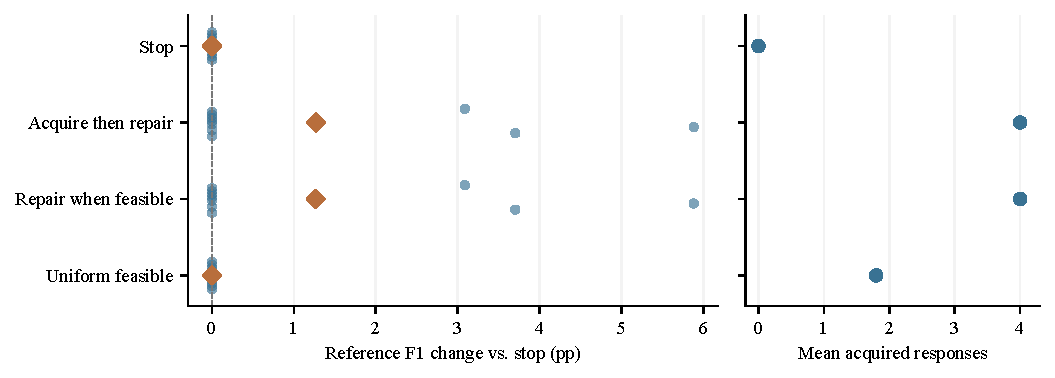
\includegraphics[width=0.94\textwidth]{figure/experiments/docred_source_pilot_round2.pdf}
\caption{Second and final development round on the same ten pairs.
F1 improves under the two repair schedules without reference losses, but all
removals use type constraints. Repeated rounds are not new test documents.}
\label{fig:docred_source_round2}
\end{figure*}
